% !TeX program = xelatex
% !TeX encoding = UTF-8
% !TeX TXS-program:compile = txs:///xelatex | txs:///xelatex
\documentclass[aspectratio=169, table, 12pt]{beamer}
% Preamble bersama seluruh slide mata kuliah ini.
% Dipanggil dari slides/sessionXX/sessionXX.tex tepat sesudah baris
% \documentclass[aspectratio=169, table, 12pt]{beamer}
% Paket tambahan yang hanya dibutuhkan satu sesi ditulis di berkas sesi itu.

\usepackage{colortbl}
\usepackage{xcolor}
\usepackage{listings}
\usepackage{tabularx}
\usepackage{booktabs}
\usepackage{tikz}
\usepackage{pgfplots}
\pgfplotsset{compat=1.18}
\usetikzlibrary{arrows.meta, positioning, calc, fit, shapes.geometric,
	shapes.multipart, backgrounds, matrix, chains, trees}

\makeatletter
\def\input@path{{../theme/}}
\makeatother
\graphicspath{{../theme/}{../../figures/}}
\usetheme{Pradita}

\definecolor{praditagreen}{RGB}{37, 113, 71}

% Tema membuat garis tabel berwarna putih. Dikembalikan agar tabel terbaca.
\arrayrulecolor{black}
\setlength{\arrayrulewidth}{0.5pt}

\lstdefinelanguage{yaml}{
	basicstyle=\ttfamily\scriptsize,
	keywordstyle=\color{blue}\bfseries,
	commentstyle=\color{gray}\itshape,
	stringstyle=\color{red},
	showstringspaces=false,
	breaklines=true,
	frame=lines,
	numbers=none,
	backgroundcolor=\color{lightgray!10},
	tabsize=2,
	morecomment=[l]{\#}
}

\lstdefinelanguage{json}{
	basicstyle=\ttfamily\scriptsize,
	stringstyle=\color{red},
	commentstyle=\color{gray},
	breaklines=true,
	showstringspaces=false,
	tabsize=2,
	numbers=none,
	frame=lines,
	backgroundcolor=\color{lightgray!10},
	string=[s]{"}{"}
}

\lstdefinelanguage{bash}{
	keywords={},
	basicstyle=\ttfamily\scriptsize,
	ndkeywords={docker, kubectl, helm, curl, git, terraform},
	ndkeywordstyle=\color{purple}\bfseries,
	sensitive=true,
	commentstyle=\color{gray},
	numbers=none,
	breaklines=true,
	frame=lines,
	backgroundcolor=\color{lightgray!10},
	tabsize=2,
	comment=[l]{\#},
	showstringspaces=false
}

\lstdefinelanguage{http}{
	keywords={GET, POST, PUT, PATCH, DELETE, HEAD, OPTIONS, HTTP},
	basicstyle=\ttfamily\scriptsize,
	keywordstyle=\color{blue}\bfseries,
	sensitive=true,
	numbers=none,
	breaklines=true,
	frame=lines,
	backgroundcolor=\color{lightgray!10},
	tabsize=2,
	showstringspaces=false
}

\subtitle{IT40613 · Digital Platform \& API Economy}
\author{\textbf{Alfa Yohannis}}


\title{\Huge Gaya API\\ \vspace{10pt} dan Pola Integrasi}
\date{Pertemuan 05}

\begin{document}
\frame{\titlepage}

\begin{frame}
  \frametitle{Isi Pertemuan}
  \vspace{14pt}
  \begin{columns}[t]
    \column{0.5\textwidth}
    {\small\tableofcontents[sections={1-4}]}

    \column{0.5\textwidth}
    {\small\tableofcontents[sections={5-9}]}
  \end{columns}
\end{frame}

\begin{frame}{\hfill}
  \centering
  \Huge{\textbf{Klinik mitra menelepon lagi.\\Aplikasi pasien menunggu lagi.\\Server kurang cepat,\\atau salah cara bicara?}}
\end{frame}

\section{Tujuan dan Konteks}

\begin{frame}{{\Large Tujuan Pembelajaran}}
  \vspace{10pt}
  \begin{itemize}
    \item Membedakan REST (\textit{Representational State Transfer}), GraphQL, \textit{event}, dan \textit{webhook} berdasarkan cara kerja dan kegunaannya.
    \item Menilai kecocokan gaya API untuk suatu kebutuhan bisnis beserta \textit{tradeoff}-nya.
    \item Memetakan integrasi yang berjalan beserta gaya dan titik masalahnya.
  \end{itemize}
\end{frame}

\begin{frame}{{\Large Diagram Konsep Bab 5}}
  \centering
  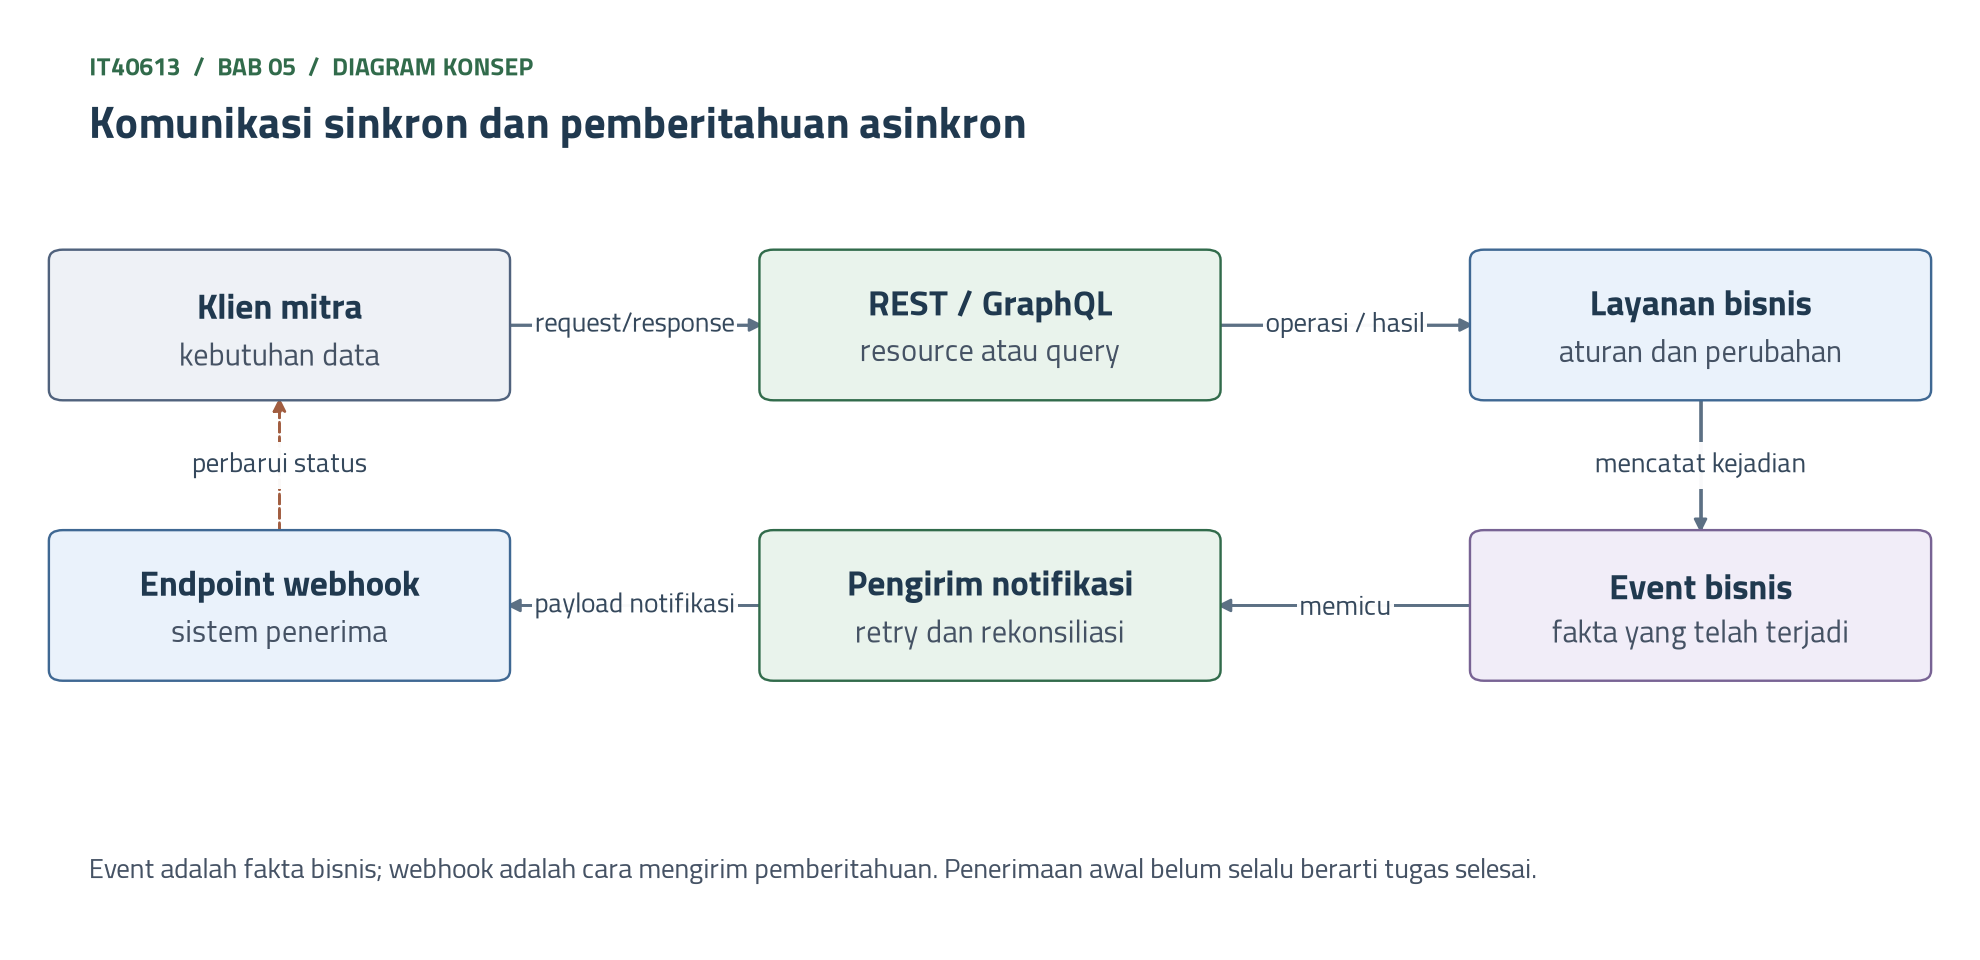
\includegraphics[width=0.96\textwidth,height=0.77\textheight,keepaspectratio]{../../figures/ch05-diagram-konsep.png}
\end{frame}

\section{Empat Cara Bertukar Data}

\begin{frame}{\hfill}
  \centering
  \Huge{\textbf{Empat Cara\\Sistem Bertukar Data}}
\end{frame}

\begin{frame}{{\Large Empat Cara dari Hohpe dan Woolf}}
  \vspace{10pt}
  \begin{itemize}
    \item Pertukaran berkas: data terkumpul, lalu diproses pada waktu tertentu.
    \item Basis data bersama: akses mudah, pemakai terikat pada struktur yang sama.
    \item Panggilan langsung: jawaban segera, pemanggil bergantung pada penyedia.
    \item Pesan: waktu pengirim dan penerima terpisah.
    \item Keempatnya boleh hidup bersama bila pemilik dan akibat gagalnya jelas.
  \end{itemize}
  \vspace{6pt}
  {\small Analogi: laporan harian, lemari arsip bersama, telepon, dan kotak surat.}
\end{frame}

\begin{frame}{{\Large Kekuatan dan Risiko Keempat Cara}}
  \footnotesize
  \begin{tabularx}{\textwidth}{>{\raggedright\arraybackslash}p{2.6cm}
      >{\raggedright\arraybackslash}X >{\raggedright\arraybackslash}X >{\raggedright\arraybackslash}p{3.3cm}}
    \hline
    \textbf{Cara} & \textbf{Kekuatan} & \textbf{Risiko} & \textbf{Contoh Medikara} \\ \hline
    Pertukaran berkas & Sederhana, cocok untuk kiriman berkala & Jeda pengiriman, salah format terlihat belakangan & INT-05: klaim mingguan ke 9 portal \\ \hline
    Basis data bersama & Data tersedia tanpa perantara & Terikat struktur tabel, akses mudah melebar & INT-03: 140 tabel terbaca, 2 tabel dibutuhkan \\ \hline
    Panggilan langsung & Jawaban segera, kesalahan terlihat & Bergantung pada ketersediaan penyedia & INT-01: kepesertaan BPJS Kesehatan \\ \hline
    Pesan & Tidak perlu hidup bersamaan & Tertunda, perlu pelacakan dan penanganan ganda & Belum ada, hasil laboratorium menjadi calon \\ \hline
  \end{tabularx}

  \vspace{6pt}
  Contoh: klaim INT-05 rata-rata menunggu 3,5 hari. Pembaruan SIMRS mengosongkan jadwal INT-03 selama 7 sampai 14 hari setahun.
\end{frame}

\begin{frame}{{\Large Inventaris Bab 4 Dibaca Ulang}}
  \small
  \begin{tabularx}{\textwidth}{>{\raggedright\arraybackslash}p{3.9cm}
      >{\raggedright\arraybackslash}X >{\raggedright\arraybackslash}p{2.0cm}}
    \hline
    \textbf{Cara} & \textbf{Baris inventaris} & \textbf{Sambungan} \\ \hline
    Pertukaran berkas & INT-04, INT-05, INT-06, INT-07, INT-08, INT-09, INT-10 & 85 \\ \hline
    Basis data bersama & INT-03 & 5 \\ \hline
    Panggilan langsung & INT-01, INT-02 & 10 \\ \hline
    Pesan & Belum ada & 0 \\ \hline
  \end{tabularx}

  \vspace{8pt}
  Akibatnya: janji ``segera'' belum mungkin dipenuhi, dan pihak yang menunggu perubahan hanya dapat bertanya berulang.

  \vspace{4pt}
  Cara bertukar data berbeda dari gaya API: REST, GraphQL, dan gRPC adalah panggilan langsung.
\end{frame}

\section{Sinkron dan Asinkron}

\begin{frame}{\hfill}
  \centering
  \Huge{\textbf{Komunikasi Sinkron\\dan Asinkron}}
\end{frame}

\begin{frame}{{\Large Siapa Menunggu Siapa}}
  \vspace{10pt}
  \begin{itemize}
    \item Sinkron: pemanggil menunggu jawaban dalam satu interaksi.
    \item Asinkron: penerimaan dan penyelesaian terjadi pada waktu berbeda.
    \item Asinkron tidak menjamin selesai: perlu ID pekerjaan, status, tenggat, dan eskalasi.
    \item Ketersediaan bergantung pada seluruh rantai, bukan layanan pertama saja.
    \item Kode 202 berarti diterima, bukan selesai.
  \end{itemize}
  \vspace{6pt}
  {\small Analogi: telepon meminta perhatian saat itu juga, surat perlu alamat dan pelacakan.}
\end{frame}

\begin{frame}{{\Large Sinkron dan Asinkron Berdampingan}}
  \centering
  \eadiagram{../../figures/ch05-sinkron-asinkron.tex}
\end{frame}

\begin{frame}{{\Large Contoh Berangka: Rantai Pemesanan dan Rekap}}
  \vspace{10pt}
  \begin{itemize}
    \item Misalkan menunggu notifikasi 5 detik: 28.000 janji temu, sekitar 39 jam per bulan.
    \item Misalkan ketersediaan 99,9, 99,5, dan 99,0 persen: rantai sinkron 98,41 persen.
    \item Sekitar 446 pemesanan gagal per bulan. Notifikasi dipisah: 99,40 persen, 168 gagal.
    \item Misalkan 36 rekap, 3 menit per rekap, batas panggilan 30 detik: selalu gagal.
    \item Solusinya kode 202, ID pekerjaan, dan pemeriksaan status.
  \end{itemize}
\end{frame}

\begin{frame}{{\Large Perbedaan yang Perlu Diperiksa}}
  \small
  \begin{tabularx}{\textwidth}{>{\raggedright\arraybackslash}p{3.6cm}
      >{\raggedright\arraybackslash}X >{\raggedright\arraybackslash}X}
    \hline
    \textbf{Unsur} & \textbf{Sinkron} & \textbf{Asinkron} \\ \hline
    Arti jawaban pertama & Hasil akhir & Permintaan diterima \\ \hline
    Bila penyedia mati & Pemanggil langsung gagal & Pekerjaan tertunda \\ \hline
    Saat beban puncak & Pemanggil ikut melambat & Antrean memanjang \\ \hline
    Yang wajib disediakan & Batas waktu yang jelas & ID, status, tenggat, eskalasi \\ \hline
    Contoh Medikara & Konfirmasi slot dokter & Rekap, pengingat, hasil tersedia \\ \hline
  \end{tabularx}

  \vspace{6pt}
  Kasus Medikara: mengunci slot wajib sinkron, pengingat boleh asinkron. Sekitar 278 pemesanan per bulan tidak lagi gagal, tetapi pengingat yang gagal harus dikirim ulang.
\end{frame}

\section{REST}

\begin{frame}{\hfill}
  \centering
  \Huge{\textbf{REST: Sumber Daya,\\Metode, dan Kode Status}}
\end{frame}

\begin{frame}{{\Large Apa Itu REST}}
  \vspace{10pt}
  \begin{itemize}
    \item Gaya arsitektur dari Fielding, bukan sekadar penamaan URL.
    \item Batasannya: klien dan server dipisah, tanpa keadaan sesi, dapat di-\textit{cache}, antarmuka seragam, berlapis.
    \item Abstraksi utama: sumber daya, yaitu informasi apa pun yang dapat diberi nama.
    \item Metode aman hanya membaca. Metode idempoten aman diulang.
    \item Kontraknya ditulis dengan OpenAPI, dibahas di Bab 9.
  \end{itemize}
  \vspace{6pt}
  {\small Analogi: jenis formulir di loket menjelaskan maksud, cap jawaban berarti sama di semua loket.}
\end{frame}

\begin{frame}{{\Large Metode HTTP Membawa Janji}}
  \small
  \begin{tabularx}{\textwidth}{>{\raggedright\arraybackslash}p{1.8cm}
      >{\raggedright\arraybackslash}X >{\raggedright\arraybackslash}p{1.3cm}
      >{\raggedright\arraybackslash}p{2.1cm} >{\raggedright\arraybackslash}X}
    \hline
    \textbf{Metode} & \textbf{Arti} & \textbf{Aman} & \textbf{Idempoten} & \textbf{Contoh Medikara} \\ \hline
    \texttt{GET} & Membaca sumber daya & Ya & Ya & Membaca jadwal dokter \\ \hline
    \texttt{POST} & Memproses, sering membuat data baru & Tidak & Tidak & Membuat janji temu \\ \hline
    \texttt{PUT} & Mengganti keadaan sumber daya & Tidak & Ya & Mengganti data kontak pasien \\ \hline
    \texttt{DELETE} & Menghapus sumber daya & Tidak & Ya & Membatalkan janji temu \\ \hline
  \end{tabularx}
\end{frame}

\begin{frame}{{\Large Kode Status Tambahan}}
  \small
  \begin{tabularx}{\textwidth}{>{\raggedright\arraybackslash}p{1.0cm}
      >{\raggedright\arraybackslash}p{3.0cm} >{\raggedright\arraybackslash}X >{\raggedright\arraybackslash}p{3.7cm}}
    \hline
    \textbf{Kode} & \textbf{Nama} & \textbf{Contoh Medikara} & \textbf{Yang bertindak} \\ \hline
    201 & Created & Janji temu dibuat, lokasinya ada di \textit{header} & Tidak ada \\ \hline
    202 & Accepted & Permintaan rekap diterima, belum selesai & Pemanggil memeriksa status \\ \hline
    409 & Conflict & Slot sudah dipakai pasien lain & Pasien memilih slot lain \\ \hline
    429 & Too Many Requests & Klinik melampaui kuota 300 per hari & Klinik menunda sesuai \texttt{Retry-After} \\ \hline
  \end{tabularx}

  \vspace{8pt}
  Bab 1 sudah memperkenalkan 200, 400, 401, 403, 404, 500, dan 503.
\end{frame}

\begin{frame}{{\Large Dua Contoh Berangka: Cache dan Janji Ganda}}
  \vspace{10pt}
  \begin{itemize}
    \item Misalkan 56.000 \texttt{GET} dan 28.000 \texttt{POST} per bulan.
    \item Misalkan separuh \texttt{GET} dilayani \textit{cache}: SIMRS terhindar dari 28.000 pembacaan.
    \item Misalkan 280 jawaban \texttt{POST} hilang, separuh sudah tersimpan: 140 janji ganda.
    \item Misalkan 6 menit per perbaikan: 14 jam per bulan, Rp10,08 juta per tahun.
    \item Kunci idempotensi mencegahnya, tetapi \texttt{Idempotency-Key} masih draf IETF.
  \end{itemize}
\end{frame}

\section{GraphQL}

\begin{frame}{\hfill}
  \centering
  \Huge{\textbf{GraphQL untuk\\Kebutuhan Data Beragam}}
\end{frame}

\begin{frame}{{\Large Apa Itu GraphQL}}
  \vspace{10pt}
  \begin{itemize}
    \item Bahasa \textit{query} dengan skema bertipe, menurut spesifikasi September 2025.
    \item Klien memilih bidang, jawabannya mengikuti bentuk permintaan.
    \item Server tetap menentukan otorisasi, biaya, dan batas kedalaman.
    \item Satu \textit{endpoint} tidak berarti satu operasi murah.
    \item Satu jawaban dapat memuat data sebagian dan daftar \textit{error}.
  \end{itemize}
  \vspace{6pt}
  {\small Analogi: daftar pesanan katering bebas dipilih, tetapi dapur tetap membatasi kapasitas.}
\end{frame}

\begin{frame}{{\Large REST dan GraphQL pada Satu Layar}}
  \centering
  \eadiagram{../../figures/ch05-rest-graphql.tex}
\end{frame}

\begin{frame}{{\Large Contoh Berangka dan Bukti Riset}}
  \vspace{10pt}
  \begin{itemize}
    \item Misalkan 3.000 layar per hari. REST: 12.000 panggilan, 90 MB. GraphQL: 3.000, 18 MB.
    \item Misalkan berurutan: 1,2 detik pada REST, 0,5 detik pada GraphQL.
    \item Brito dkk.: tujuh sistem, median turun 94 persen bidang, 99 persen byte.
    \item Brito dan Valente: 22 mahasiswa, median 6 menit lawan 9 menit.
    \item Keduanya mengukur sisi klien, bukan biaya menjaga server.
  \end{itemize}
\end{frame}

\begin{frame}{{\Large Risiko di Sisi Server}}
  \vspace{10pt}
  \begin{itemize}
    \item Misalkan 18 klinik, 500 pasien, 5 kunjungan, 4 hasil: 180.000 objek dari satu panggilan.
    \item Misalkan 1 milidetik per objek: server bekerja 180 detik.
    \item Hartig dan P{\'e}rez: ukuran jawaban dapat terlalu besar untuk skenario internet.
    \item Cha dkk.: manajemen API tradisional tidak cukup, biaya perlu ditaksir sebelum jalan.
    \item Pengendalian: halaman, kedalaman, lebar, laju, dan bobot biaya.
  \end{itemize}
\end{frame}

\begin{frame}{{\Large REST dan GraphQL untuk Keputusan}}
  \footnotesize
  \begin{tabularx}{\textwidth}{>{\raggedright\arraybackslash}p{3.2cm}
      >{\raggedright\arraybackslash}X >{\raggedright\arraybackslash}X}
    \hline
    \textbf{Unsur} & \textbf{REST} & \textbf{GraphQL} \\ \hline
    Bentuk jawaban & Ditetapkan penyedia per sumber daya & Dipilih klien dalam batas skema \\ \hline
    Kontrak & OpenAPI, dibahas di Bab 9 & Skema bertipe, ditinjau bersama \\ \hline
    \textit{Cache} & Memakai \textit{cache} HTTP per alamat & Satu alamat, perlu cara lain \\ \hline
    Pengendalian beban & Kuota per \textit{endpoint} & Batas kedalaman, lebar, dan biaya \textit{query} \\ \hline
    Pemantauan & Kode status per panggilan & Isi jawaban ikut dibaca \\ \hline
    Cocok untuk & Operasi jelas, mitra banyak dan beragam & Layar beragam, klien dikenal \\ \hline
  \end{tabularx}
\end{frame}

\section{Event dan Webhook}

\begin{frame}{\hfill}
  \centering
  \Huge{\textbf{Event dan Webhook}}
\end{frame}

\begin{frame}{{\Large Fakta dan Cara Mengantarnya}}
  \vspace{10pt}
  \begin{itemize}
    \item \textit{Event}: catatan bahwa sesuatu telah terjadi, yaitu fakta bisnis.
    \item \textit{Webhook}: salah satu cara mengirim pemberitahuan ke URL penerima.
    \item \textit{Polling}: penerima meminta status berulang.
    \item Fakta yang sama dapat diantar lewat \textit{webhook}, pesan, atau dibaca lewat \textit{polling}.
    \item Pemberitahuan dapat terlambat atau terkirim ulang.
  \end{itemize}
  \vspace{6pt}
  {\small Analogi: papan pengumuman harus diperiksa, petugas pengantar datang bila ada surat.}
\end{frame}

\begin{frame}{{\Large Polling dan Webhook pada Klinik Mitra}}
  \centering
  \eadiagram{../../figures/ch05-polling-webhook.tex}
\end{frame}

\begin{frame}{{\Large Hitungan pada 40 Klinik Mitra}}
  \small
  Misalkan 10 persen dari 60 kunjungan per hari per klinik: 240 hasil per hari, 20 per jam.

  \vspace{6pt}
  \begin{tabularx}{\textwidth}{>{\raggedright\arraybackslash}p{3.8cm}
      >{\raggedright\arraybackslash}X >{\raggedright\arraybackslash}X}
    \hline
    \textbf{Unsur} & \textbf{\textit{Polling} tiap 5 menit} & \textbf{\textit{Webhook} dan rekonsiliasi} \\ \hline
    Permintaan per hari & 5.760 & 725 \\ \hline
    Tunda rata-rata & 2,5 menit & Misalkan beberapa detik \\ \hline
    Kuota per klinik & 324 dari 300, melampaui & 192 dari 300, aman \\ \hline
    Bila penerima mati & Bertanya lagi setelah hidup & Pengirim mengulang, rekonsiliasi menutup sisanya \\ \hline
  \end{tabularx}
\end{frame}

\begin{frame}{{\Large Isi Kontrak Pemberitahuan}}
  \vspace{10pt}
  \begin{itemize}
    \item Pengenal kejadian: sama pada setiap pengulangan, untuk mendeteksi ganda.
    \item Tanda tangan dan waktu kirim: membuktikan pengirim, menolak serangan ulang.
    \item Arti berhasil: kode 2xx. GitHub meminta jawaban dalam 10 detik.
    \item Jadwal \textit{retry}: berhari-hari dengan selang yang makin panjang.
    \item Rekonsiliasi: penerima mencocokkan status secara berkala.
  \end{itemize}
  \vspace{6pt}
  {\small Rujukan: Standard Webhooks, CloudEvents 1.0.2, dan AsyncAPI 3.1 untuk kontrak pesan.}
\end{frame}

\begin{frame}{{\Large Kasus Medikara: Hasil Laboratorium}}
  \vspace{10pt}
  \begin{itemize}
    \item Misalkan 30 persen hasil diikuti telepon: 72 telepon per hari, 180 jam per bulan.
    \item Biaya telepon: Rp10,8 juta per bulan, Rp129,6 juta per tahun.
    \item Satu API hasil dengan \textit{webhook}: Rp45 juta per tahun, selisih Rp84,6 juta.
    \item \textit{Payload} tanpa isi hasil: tambah 240 \texttt{GET}, total 965 per hari.
    \item Klinik yang belum punya \textit{endpoint}: \textit{polling} tiap 6 menit.
  \end{itemize}
\end{frame}

\section{Memilih Gaya API}

\begin{frame}{\hfill}
  \centering
  \Huge{\textbf{Memilih Gaya API}}
\end{frame}

\begin{frame}{{\Large Kriteria dan gRPC sebagai Pembanding}}
  \vspace{10pt}
  \begin{itemize}
    \item Kriteria: kebutuhan jawaban, toleransi tunda, pola beban, ragam data, kemampuan mitra.
    \item Satu produk API boleh memakai lebih dari satu gaya.
    \item gRPC: kerangka RPC, kontrak lebih dulu, memakai HTTP/2, aliran data dua arah.
    \item Klien peramban memerlukan gRPC-Web lewat \textit{proxy} khusus.
    \item Keterikatan dan titik kegagalan tunggal ikut dinilai.
  \end{itemize}
  \vspace{6pt}
  {\small Analogi: motor, mobil boks, dan truk punya perjalanannya masing-masing.}
\end{frame}

\begin{frame}{{\Large Peta Keputusan Gaya API}}
  \centering
  \resizebox{!}{0.8\textheight}{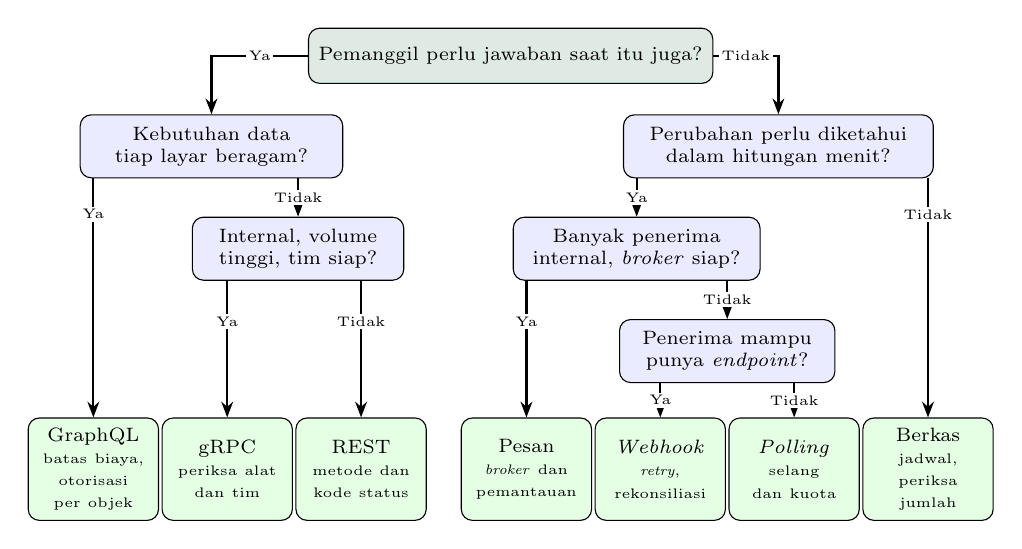
\begin{tikzpicture}[
  font=\scriptsize,
  execute at begin node={\hyphenpenalty=10000\exhyphenpenalty=10000},
  tanya/.style={draw, rounded corners, fill=blue!8, align=center, minimum height=0.8cm},
  awal/.style={draw, rounded corners, fill=praditagreen!15, align=center, minimum height=0.7cm, text width=4.9cm},
  daun/.style={draw, rounded corners, fill=green!10, text width=1.42cm, minimum height=1.3cm, align=center},
  ket/.style={font=\tiny, fill=white, inner sep=1pt},
  panah/.style={-{Stealth[length=2mm]}, thick}
]
  % Pertanyaan pertama memisahkan kebutuhan jawaban segera dari pemberitahuan.
  \node[awal] (q1) at (6.1,0) {Pemanggil perlu jawaban saat itu juga?};
  \node[tanya, text width=3.1cm] (q2) at (2.3,-1.15) {Kebutuhan data tiap layar beragam?};
  \node[tanya, text width=3.7cm] (q4) at (9.5,-1.15) {Perubahan perlu diketahui dalam hitungan menit?};
  \node[tanya, text width=2.45cm] (q3) at (3.4,-2.45) {Internal, volume tinggi, tim siap?};
  \node[tanya, text width=2.9cm] (q5) at (7.7,-2.45) {Banyak penerima internal, \textit{broker} siap?};
  \node[tanya, text width=2.5cm] (q6) at (8.85,-3.75) {Penerima mampu punya \textit{endpoint}?};

  % Daun keputusan: tiap pilihan membawa syarat yang wajib ditulis di kontrak.
  \node[daun] (graphql) at (0.8,-5.25) {GraphQL\\{\tiny\mdseries batas biaya, otorisasi per objek}};
  \node[daun] (grpc) at (2.5,-5.25) {gRPC\\{\tiny\mdseries periksa alat dan tim}};
  \node[daun] (rest) at (4.2,-5.25) {REST\\{\tiny\mdseries metode dan kode status}};
  \node[daun] (pesan) at (6.3,-5.25) {Pesan\\{\tiny\mdseries \textit{broker} dan pemantauan}};
  \node[daun] (webhook) at (8.0,-5.25) {\textit{Webhook}\\{\tiny\mdseries \textit{retry}, rekonsiliasi}};
  \node[daun] (polling) at (9.7,-5.25) {\textit{Polling}\\{\tiny\mdseries selang dan kuota}};
  \node[daun] (berkas) at (11.4,-5.25) {Berkas\\{\tiny\mdseries jadwal, periksa jumlah}};

  % Garis keputusan.
  \draw[panah] (q1.west) -| node[ket, pos=0.25] {Ya} (q2.north);
  \draw[panah] (q1.east) -| node[ket, pos=0.25] {Tidak} (q4.north);
  \draw[panah] (graphql.north |- q2.south) -- node[ket, pos=0.15] {Ya} (graphql.north);
  \draw[panah] (q3.north |- q2.south) -- node[ket] {Tidak} (q3.north);
  \draw[panah] (grpc.north |- q3.south) -- node[ket, pos=0.3] {Ya} (grpc.north);
  \draw[panah] (rest.north |- q3.south) -- node[ket, pos=0.3] {Tidak} (rest.north);
  \draw[panah] (q5.north |- q4.south) -- node[ket] {Ya} (q5.north);
  \draw[panah] (berkas.north |- q4.south) -- node[ket, pos=0.15] {Tidak} (berkas.north);
  \draw[panah] (pesan.north |- q5.south) -- node[ket, pos=0.3] {Ya} (pesan.north);
  \draw[panah] (q6.north |- q5.south) -- node[ket] {Tidak} (q6.north);
  \draw[panah] (webhook.north |- q6.south) -- node[ket] {Ya} (webhook.north);
  \draw[panah] (polling.north |- q6.south) -- node[ket] {Tidak} (polling.north);
\end{tikzpicture}
}
\end{frame}

\begin{frame}{{\Large Dua Contoh Berangka: Broker dan gRPC}}
  \vspace{10pt}
  \begin{itemize}
    \item REST dan \textit{webhook}: misalkan 16 jam per klinik, tahun pertama Rp83,4 juta.
    \item \textit{Broker}: misalkan 120 jam per klinik dan lapisan Rp300 juta, tahun pertama Rp633 juta.
    \item Selisih Rp549,6 juta, ditinjau lagi bila banyak layanan internal butuh \textit{event} sama.
    \item gRPC: misalkan 100.000 panggilan per hari, hemat 140 MB, pelatihan Rp12 juta.
    \item Pada volume ini gRPC belum sepadan.
  \end{itemize}
\end{frame}

\begin{frame}{{\Large Peta Integrasi Medikara}}
  \centering
  \resizebox{!}{0.8\textheight}{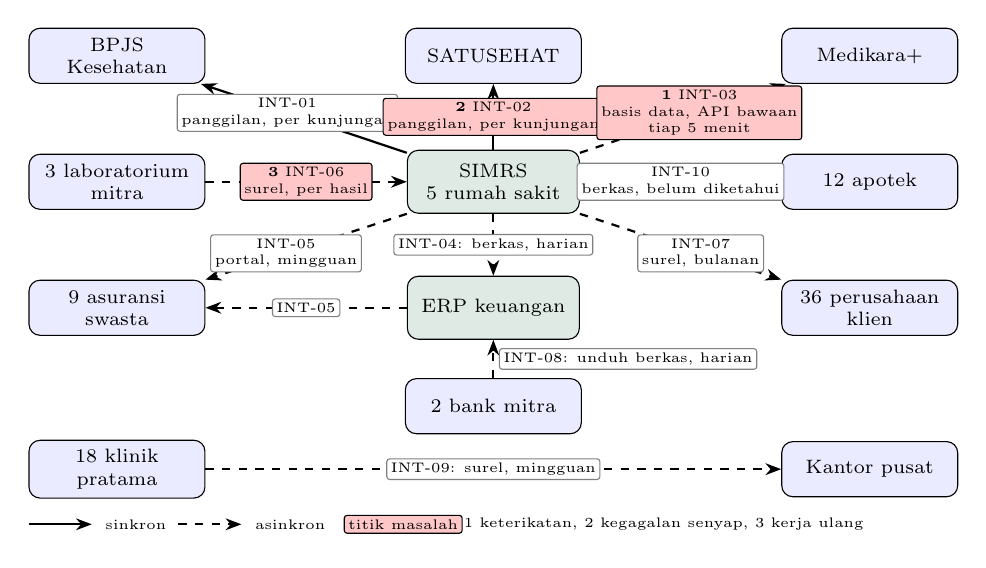
\begin{tikzpicture}[
  font=\scriptsize,
  execute at begin node={\hyphenpenalty=10000\exhyphenpenalty=10000},
  inti/.style={draw, rounded corners, fill=praditagreen!15, text width=1.95cm, minimum height=0.8cm, align=center},
  pihak/.style={draw, rounded corners, fill=blue!8, text width=2.0cm, minimum height=0.7cm, align=center},
  label/.style={draw=gray, solid, thin, rounded corners=1pt, fill=white, font=\tiny, align=center, inner sep=1.5pt},
  masalah/.style={draw, solid, thin, rounded corners=1pt, fill=red!22, font=\tiny, align=center, inner sep=1.5pt},
  ket/.style={font=\tiny, anchor=west},
  panah/.style={-{Stealth[length=2mm]}, thick},
  jeda/.style={-{Stealth[length=2mm]}, thick, dashed}
]
  % Dua sistem inti Medikara berada di tengah peta.
  \node[inti] (simrs) at (5.9,0) {SIMRS\\5 rumah sakit};
  \node[inti] (erp) at (5.9,-1.6) {ERP keuangan};

  % Pihak dan sistem di sekelilingnya, dengan ID yang sama seperti inventaris Bab 4.
  \node[pihak] (bpjs) at (1.12,1.6) {BPJS Kesehatan};
  \node[pihak] (sehat) at (5.9,1.6) {SATUSEHAT};
  \node[pihak] (plus) at (10.68,1.6) {Medikara+};
  \node[pihak] (lab) at (1.12,0) {3 laboratorium mitra};
  \node[pihak] (apotek) at (10.68,0) {12 apotek};
  \node[pihak] (asuransi) at (1.12,-1.6) {9 asuransi swasta};
  \node[pihak] (usaha) at (10.68,-1.6) {36 perusahaan klien};
  \node[pihak] (bank) at (5.9,-2.85) {2 bank mitra};
  \node[pihak] (klinik) at (1.12,-3.65) {18 klinik pratama};
  \node[pihak] (pusat) at (10.68,-3.65) {Kantor pusat};

  % Garis penuh sinkron, garis putus asinkron.
  \draw[panah] (simrs) -- node[label, pos=0.58] {INT-01\\panggilan, per kunjungan} (bpjs);
  \draw[panah] (simrs) -- node[masalah] {\textbf{2} INT-02\\panggilan, per kunjungan} (sehat);
  \draw[jeda] (simrs) -- node[masalah, pos=0.58] {\textbf{1} INT-03\\basis data, API bawaan\\tiap 5 menit} (plus);
  \draw[jeda] (simrs) -- node[label] {INT-04: berkas, harian} (erp);
  \draw[jeda] (simrs.south west) -- node[label, pos=0.6] {INT-05\\portal, mingguan} (asuransi.north east);
  \draw[jeda] (erp) -- node[label] {INT-05} (asuransi);
  \draw[jeda] (lab) -- node[masalah] {\textbf{3} INT-06\\surel, per hasil} (simrs);
  \draw[jeda] (simrs.south east) -- node[label, pos=0.6] {INT-07\\surel, bulanan} (usaha.north west);
  \draw[jeda] (bank) -- node[label, right=2pt] {INT-08: unduh berkas, harian} (erp);
  \draw[jeda] (klinik) -- node[label] {INT-09: surel, mingguan} (pusat);
  \draw[jeda] (simrs) -- node[label] {INT-10\\berkas, belum diketahui} (apotek);

  % Keterangan peta.
  \draw[panah] (0.0,-4.35) -- (0.8,-4.35);
  \node[ket] at (0.85,-4.35) {sinkron};
  \draw[jeda] (1.9,-4.35) -- (2.7,-4.35);
  \node[ket] at (2.75,-4.35) {asinkron};
  \node[masalah, anchor=west] at (4.0,-4.35) {titik masalah};
  \node[ket] at (5.4,-4.35) {1 keterikatan, 2 kegagalan senyap, 3 kerja ulang};
\end{tikzpicture}
}
\end{frame}

\begin{frame}{{\Large Kasus Medikara: Tiga Titik Masalah}}
  \vspace{10pt}
  \begin{itemize}
    \item INT-03, keterikatan: 138 tabel di luar kebutuhan, jadwal kosong 7 sampai 14 hari.
    \item INT-02, kegagalan senyap: sekitar 4 persen kunjungan klinik belum terkirim.
    \item INT-06, kerja ulang: 1.100 per bulan, 110 jam, Rp79,2 juta per tahun.
    \item INT-05 ditunda: akarnya format, ditangani lewat kontrak Bab 9.
    \item Ketiga titik ditelusuri lagi pada Bab 6 dan Bab 7.
  \end{itemize}
\end{frame}

\section{Aktivitas}

\begin{frame}{{\Large Aktivitas: Peta Integrasi Saat Ini}}
  \vspace{10pt}
  \begin{itemize}
    \item Gambar peta dari inventaris Pertemuan 4, ID tidak diganti.
    \item Label tiap garis: gaya, frekuensi, arah, sinkron atau asinkron.
    \item Non-teknis menandai antrean, kerja ulang, dan laporan terlambat.
    \item Teknis menilai keterikatan dan titik kegagalan tunggal.
    \item Luaran C2: peta dan tiga titik masalah. Berkas di \berkas{sources/chapter05/}.
  \end{itemize}
  \vspace{6pt}
  {\small Kriteria: konsep 25\%, bukti 30\%, alasan dan pengorbanan 30\%, keterbacaan 15\%.}
\end{frame}

\section{Ringkasan dan Latihan}

\begin{frame}{{\Large Ringkasan}}
  \vspace{10pt}
  \begin{itemize}
    \item Sebanyak 85 dari 100 sambungan Medikara memakai berkas, dan belum ada yang memakai pesan.
    \item Asinkron memisahkan diterima dari selesai, tetapi konfirmasi slot tetap sinkron.
    \item REST menjanjikan akibat lewat metode. GraphQL memindahkan biaya ke server.
    \item \textit{Event} adalah fakta, \textit{webhook} adalah cara mengantarnya.
    \item Gaya API menentukan siapa menunggu siapa, dan siapa menanggung akibat kegagalan.
  \end{itemize}
\end{frame}

\begin{frame}{{\Large Latihan}}
  \vspace{10pt}
  \begin{enumerate}
    \item Klinik mitra perlu segera tahu ketika hasil laboratorium selesai. Bandingkan \textit{polling} lewat REST dan \textit{webhook}, lalu pilih salah satu beserta alasannya.
    \item Jelaskan dalam bahasa non-teknis perbedaan komunikasi sinkron dan asinkron, dengan contoh dari layanan rumah sakit.
    \item Tentukan kapan GraphQL lebih tepat daripada REST, dan kapan GraphQL justru menambah risiko.
  \end{enumerate}
\end{frame}

\end{document}
